% Options for packages loaded elsewhere
\PassOptionsToPackage{unicode}{hyperref}
\PassOptionsToPackage{hyphens}{url}
\PassOptionsToPackage{dvipsnames,svgnames,x11names}{xcolor}
%
\documentclass[
]{article}

\usepackage{amsmath,amssymb}
\usepackage{iftex}
\ifPDFTeX
  \usepackage[T1]{fontenc}
  \usepackage[utf8]{inputenc}
  \usepackage{textcomp} % provide euro and other symbols
\else % if luatex or xetex
  \usepackage{unicode-math}
  \defaultfontfeatures{Scale=MatchLowercase}
  \defaultfontfeatures[\rmfamily]{Ligatures=TeX,Scale=1}
\fi
\usepackage{lmodern}
\ifPDFTeX\else  
    % xetex/luatex font selection
\fi
% Use upquote if available, for straight quotes in verbatim environments
\IfFileExists{upquote.sty}{\usepackage{upquote}}{}
\IfFileExists{microtype.sty}{% use microtype if available
  \usepackage[]{microtype}
  \UseMicrotypeSet[protrusion]{basicmath} % disable protrusion for tt fonts
}{}
\makeatletter
\@ifundefined{KOMAClassName}{% if non-KOMA class
  \IfFileExists{parskip.sty}{%
    \usepackage{parskip}
  }{% else
    \setlength{\parindent}{0pt}
    \setlength{\parskip}{6pt plus 2pt minus 1pt}}
}{% if KOMA class
  \KOMAoptions{parskip=half}}
\makeatother
\usepackage{xcolor}
\ifLuaTeX
  \usepackage{luacolor}
  \usepackage[soul]{lua-ul}
\else
  \usepackage{soul}
  
\fi
\setlength{\emergencystretch}{3em} % prevent overfull lines
\setcounter{secnumdepth}{5}
% Make \paragraph and \subparagraph free-standing
\makeatletter
\ifx\paragraph\undefined\else
  \let\oldparagraph\paragraph
  \renewcommand{\paragraph}{
    \@ifstar
      \xxxParagraphStar
      \xxxParagraphNoStar
  }
  \newcommand{\xxxParagraphStar}[1]{\oldparagraph*{#1}\mbox{}}
  \newcommand{\xxxParagraphNoStar}[1]{\oldparagraph{#1}\mbox{}}
\fi
\ifx\subparagraph\undefined\else
  \let\oldsubparagraph\subparagraph
  \renewcommand{\subparagraph}{
    \@ifstar
      \xxxSubParagraphStar
      \xxxSubParagraphNoStar
  }
  \newcommand{\xxxSubParagraphStar}[1]{\oldsubparagraph*{#1}\mbox{}}
  \newcommand{\xxxSubParagraphNoStar}[1]{\oldsubparagraph{#1}\mbox{}}
\fi
\makeatother


\providecommand{\tightlist}{%
  \setlength{\itemsep}{0pt}\setlength{\parskip}{0pt}}\usepackage{longtable,booktabs,array}
\usepackage{calc} % for calculating minipage widths
% Correct order of tables after \paragraph or \subparagraph
\usepackage{etoolbox}
\makeatletter
\patchcmd\longtable{\par}{\if@noskipsec\mbox{}\fi\par}{}{}
\makeatother
% Allow footnotes in longtable head/foot
\IfFileExists{footnotehyper.sty}{\usepackage{footnotehyper}}{\usepackage{footnote}}
\makesavenoteenv{longtable}
\usepackage{graphicx}
\makeatletter
\def\maxwidth{\ifdim\Gin@nat@width>\linewidth\linewidth\else\Gin@nat@width\fi}
\def\maxheight{\ifdim\Gin@nat@height>\textheight\textheight\else\Gin@nat@height\fi}
\makeatother
% Scale images if necessary, so that they will not overflow the page
% margins by default, and it is still possible to overwrite the defaults
% using explicit options in \includegraphics[width, height, ...]{}
\setkeys{Gin}{width=\maxwidth,height=\maxheight,keepaspectratio}
% Set default figure placement to htbp
\makeatletter
\def\fps@figure{htbp}
\makeatother
% definitions for citeproc citations
\NewDocumentCommand\citeproctext{}{}
\NewDocumentCommand\citeproc{mm}{%
  \begingroup\def\citeproctext{#2}\cite{#1}\endgroup}
\makeatletter
 % allow citations to break across lines
 \let\@cite@ofmt\@firstofone
 % avoid brackets around text for \cite:
 \def\@biblabel#1{}
 \def\@cite#1#2{{#1\if@tempswa , #2\fi}}
\makeatother
\newlength{\cslhangindent}
\setlength{\cslhangindent}{1.5em}
\newlength{\csllabelwidth}
\setlength{\csllabelwidth}{3em}
\newenvironment{CSLReferences}[2] % #1 hanging-indent, #2 entry-spacing
 {\begin{list}{}{%
  \setlength{\itemindent}{0pt}
  \setlength{\leftmargin}{0pt}
  \setlength{\parsep}{0pt}
  % turn on hanging indent if param 1 is 1
  \ifodd #1
   \setlength{\leftmargin}{\cslhangindent}
   \setlength{\itemindent}{-1\cslhangindent}
  \fi
  % set entry spacing
  \setlength{\itemsep}{#2\baselineskip}}}
 {\end{list}}
\usepackage{calc}
\newcommand{\CSLBlock}[1]{\hfill\break\parbox[t]{\linewidth}{\strut\ignorespaces#1\strut}}
\newcommand{\CSLLeftMargin}[1]{\parbox[t]{\csllabelwidth}{\strut#1\strut}}
\newcommand{\CSLRightInline}[1]{\parbox[t]{\linewidth - \csllabelwidth}{\strut#1\strut}}
\newcommand{\CSLIndent}[1]{\hspace{\cslhangindent}#1}

\makeatletter
\@ifpackageloaded{tcolorbox}{}{\usepackage[skins,breakable]{tcolorbox}}
\@ifpackageloaded{fontawesome5}{}{\usepackage{fontawesome5}}
\definecolor{quarto-callout-color}{HTML}{909090}
\definecolor{quarto-callout-note-color}{HTML}{0758E5}
\definecolor{quarto-callout-important-color}{HTML}{CC1914}
\definecolor{quarto-callout-warning-color}{HTML}{EB9113}
\definecolor{quarto-callout-tip-color}{HTML}{00A047}
\definecolor{quarto-callout-caution-color}{HTML}{FC5300}
\definecolor{quarto-callout-color-frame}{HTML}{acacac}
\definecolor{quarto-callout-note-color-frame}{HTML}{4582ec}
\definecolor{quarto-callout-important-color-frame}{HTML}{d9534f}
\definecolor{quarto-callout-warning-color-frame}{HTML}{f0ad4e}
\definecolor{quarto-callout-tip-color-frame}{HTML}{02b875}
\definecolor{quarto-callout-caution-color-frame}{HTML}{fd7e14}
\makeatother
\makeatletter
\@ifpackageloaded{caption}{}{\usepackage{caption}}
\AtBeginDocument{%
\ifdefined\contentsname
  \renewcommand*\contentsname{Table of contents}
\else
  \newcommand\contentsname{Table of contents}
\fi
\ifdefined\listfigurename
  \renewcommand*\listfigurename{List of Figures}
\else
  \newcommand\listfigurename{List of Figures}
\fi
\ifdefined\listtablename
  \renewcommand*\listtablename{List of Tables}
\else
  \newcommand\listtablename{List of Tables}
\fi
\ifdefined\figurename
  \renewcommand*\figurename{Figure}
\else
  \newcommand\figurename{Figure}
\fi
\ifdefined\tablename
  \renewcommand*\tablename{Table}
\else
  \newcommand\tablename{Table}
\fi
}
\@ifpackageloaded{float}{}{\usepackage{float}}
\floatstyle{ruled}
\@ifundefined{c@chapter}{\newfloat{codelisting}{h}{lop}}{\newfloat{codelisting}{h}{lop}[chapter]}
\floatname{codelisting}{Listing}
\newcommand*\listoflistings{\listof{codelisting}{List of Listings}}
\makeatother
\makeatletter
\makeatother
\makeatletter
\@ifpackageloaded{caption}{}{\usepackage{caption}}
\@ifpackageloaded{subcaption}{}{\usepackage{subcaption}}
\makeatother
\ifLuaTeX
  \usepackage{selnolig}  % disable illegal ligatures
\fi
\usepackage{bookmark}

\IfFileExists{xurl.sty}{\usepackage{xurl}}{} % add URL line breaks if available
\urlstyle{same} % disable monospaced font for URLs
\hypersetup{
  pdftitle={Navigating food web prediction; assumptions, rationale, and methods},
  pdfauthor={Tanya Strydom; Jennifer A. Dunne; Timothée Poisot; Andrew P. Beckerman},
  pdfkeywords={food web, network construction, scientific ignorance},
  colorlinks=true,
  linkcolor={blue},
  filecolor={Maroon},
  citecolor={Blue},
  urlcolor={Blue},
  pdfcreator={LaTeX via pandoc}}


\title{Navigating food web prediction; assumptions, rationale, and
methods}
\author{Tanya Strydom %
%
\textsuperscript{%
%
1%
}%
; Jennifer A. Dunne %
%
\textsuperscript{%
%
2%
}%
; Timothée Poisot %
%
\textsuperscript{%
3,%
4%
}%
; Andrew P. Beckerman %
%
\textsuperscript{%
%
1%
}%
}
\date{2024-05-09}

\usepackage{setspace}
\usepackage[left,pagewise]{lineno}
\usepackage[letterpaper]{geometry}

\usepackage[nolists,noheads,markers]{endfloat}
\geometry{margin=2.5cm}

\begin{document}

\thispagestyle{empty}
{\bfseries\sffamily\Large Navigating food web prediction; assumptions,
rationale, and methods}
\vfil
Tanya Strydom %
%
\textsuperscript{%
%
1%
}%
; Jennifer A. Dunne %
%
\textsuperscript{%
%
2%
}%
; Timothée Poisot %
%
\textsuperscript{%
3,%
4%
}%
; Andrew P. Beckerman %
%
\textsuperscript{%
%
1%
}%

\vfil
{\small
\textbf{Abstract:} Although it has been acknowledged that communities
consist not only of co-occurring species but that they also interact
being able to quantify those interactions and assemble them into
interaction networks has been a limiting factor in the integration of
network ecology into other fields of ecology. As the field of network
ecology has matured there has been an accompanying expansion in the
development of theory and tools that are centred around generating
networks or predicting the interactions between species. Notably many of
these tools have been developed with different underlying philosophies,
ideas, and mechanisms as to what structures the interactions between
species. It is thus critically important that those wanting to adopt
these network generating tools be aware of how the the specific
questions being asked maps to the underlying assumptions made when
generating networks, as well as the limitations of how the
networks/interactions are delimited. Here we provide an overview of the
canonical network generating models, comparing and contrasting the
underlying assumptions, data requirements, and resulting network
predictions made by the different families in an attempt to provide
guidance for those interested in adopting the generation of networks
into their workflow. {[}R1. a discussion on the underlying assumptions
we are making when we delimit a network{]}. {[}R2. an overview of how
the different model families differ - ordination space/benchmarking{]}.
{[}R3. identifying the relevant questions/bodies of theory that the
networks generated by different families are suited to answer{]}. When
choosing to construct an interaction network the researcher is faced
with many assumptions and considerations that should be made and it is
important to be aware of these limitations to avoid constructing
(something poetic to capture the idea of falsity/false idols). Being
aware of these choices is particularly important as the availability of
these tools grows and network ecology starts to be adopted into other
aspects of ecology and conservation biology.
\vfil
\textbf{Keywords:} %
food web, network construction, %
scientific ignorance%
}
\clearpage
\setcounter{page}{1}
\doublespacing
\linenumbers

Although there is a growing consensus that species interaction networks
are an important facet of understanding biodiversity (underpinning some
of the key dimensions of biodiversity??), yet it is also a field where
we are lacking in real world data {[}1{]}, and broader understanding
(Eltonian shortfall). Because of this overall lack of data (and extreme
difficulty in generating it {[}2,3{]}) we as researchers find ourselves
having to predict/construct networks using a modelling approach. The
problem with that is that there are as many models as there are ways to
define food webs and although there have been attempts to compare some
of the more canonical models in terms of their performance {[}4,5{]}
there is a distinct lack of discussion and resulting awareness of the
different model families and how they are embedding different
philosophies.

It can be argued that the interaction between species (or individuals)
is one of the main determinants of the emergent properties that are
studied in other fields of ecology, \emph{e.g.,} the range of plant will
be determined by the range of its pollinator, and although the
importance of species interactions and the resulting networks that they
form has been an acknowledged part of the ecological canon since the
penning of the `entangled bank' {[}6{]}, the adoption of network ecology
into other disciplines of ecology has been limited. This has primarily
been driven by two limitations; firstly, it is extremely challenging to
actually record species interactions in the field {[}2,3{]}, which has
resulted in a limited coverage of `real world' interaction data {[}1{]},
and secondly has been the need to develop terminology and tools that
help us to construct, conceptualise, and analyse these networks.
Although recording interactions in the field remains a challenge, the
development of both practical tools {[}\emph{i.e.,} tools that help us
to record or measure interactions, 7{]}, as well as discussions around
the development of tools to predict or infer them {[}8,9{]}, has allowed
us to begin filling in these `global gaps', albeit in a, potentially,
more synthetic manner {[}10{]}. Additionally, there has been extensive
development in in the ways in which we formalise networks {[}11,12{]},
and the tools and language that we use to quantify the structure and
properties of networks {[}13{]}. All together these tools mean that, as
a field, network ecology can (and should) be integrated into the broader
fields of ecology {[}\emph{e.g.,} 14{]} and conservation biology
{[}\emph{e.g.,} 15{]}. However (as with any new tool or model), it is
important that one has a firm grasp of how the underlying philosophy
that underpins the construction of networks (particularly synthetic
ones) can have an impact on the interpretation of the questions being
asked. In this manuscript we will discuss three themes that should help
provide clarity and understanding for those wishing to take a step into
network (particularly food web) ecology this includes; thinking about
and understanding the underlying assumptions that are made when we
attempt to delimit and describe a food webs, a synthesis of the
different families of tools that are commonly used to construct food
webs, and a discussion linking network ecology to some of the
outstanding questions in ecology.

\begin{figure}

\centering{

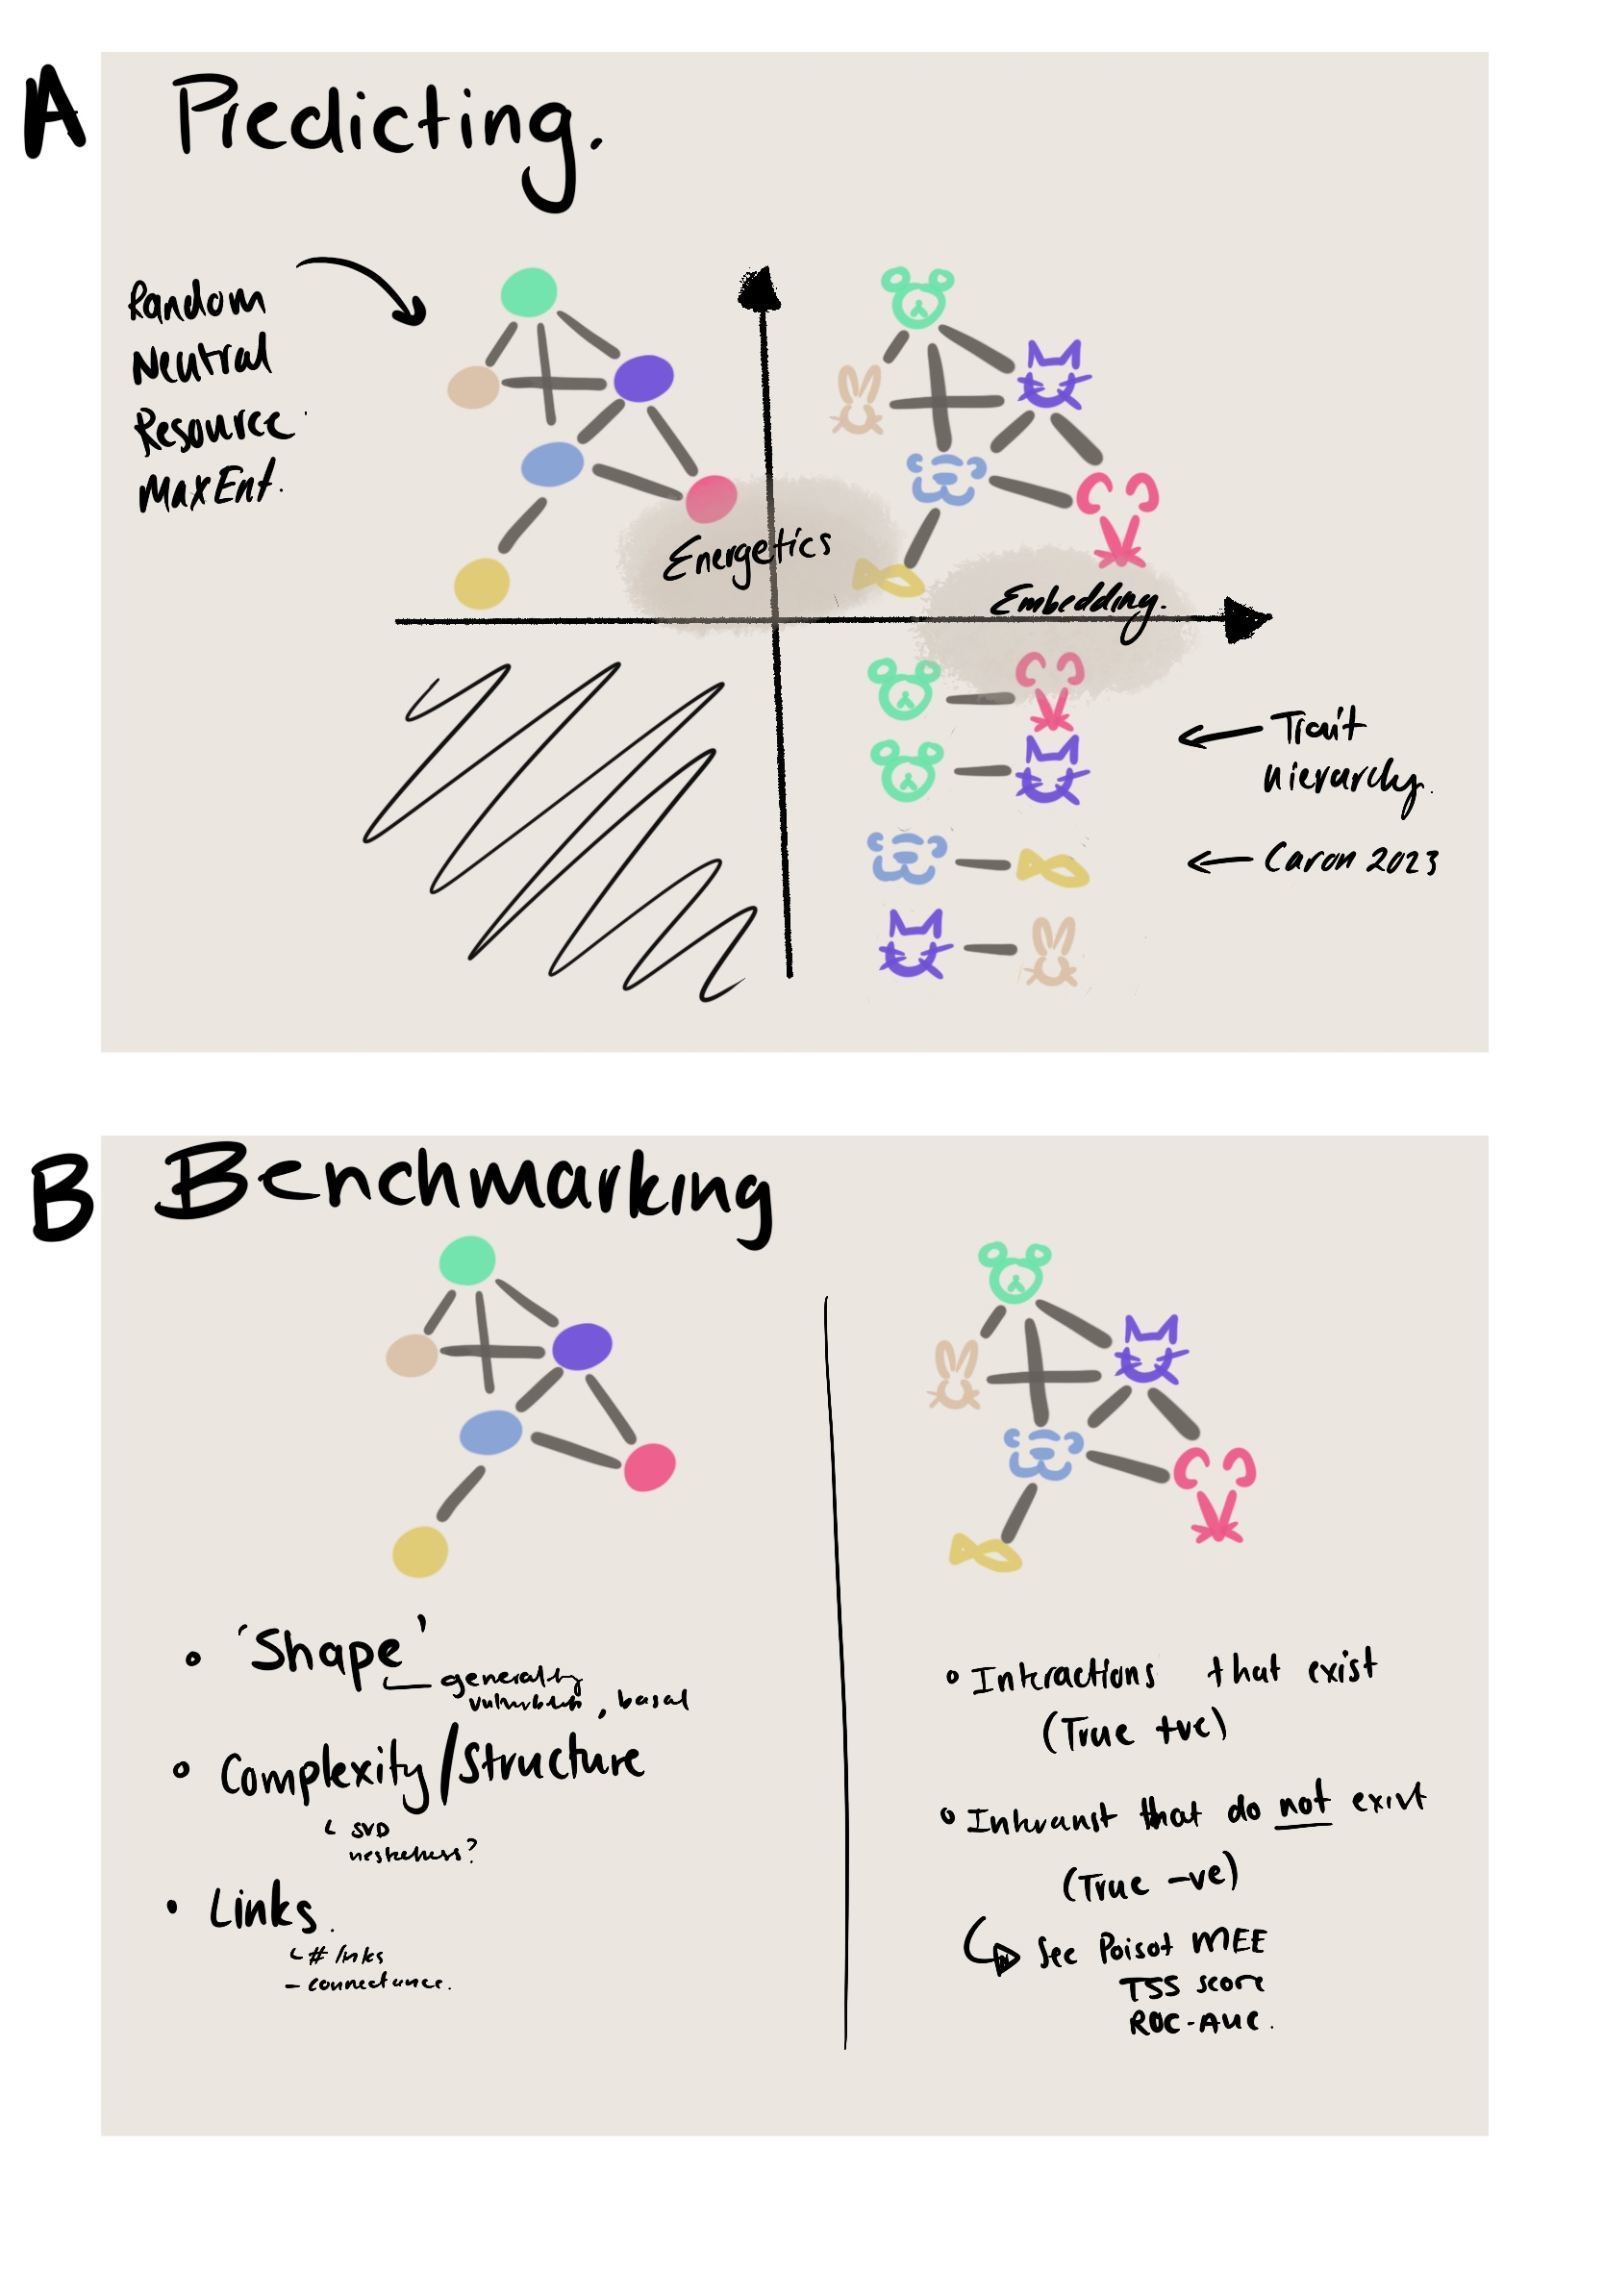
\includegraphics{images/concept.jpeg}

}

\caption{\label{fig-concept}Conceptual figure of the `network
prediction'. Panel A shows where the model families fall in the the
context of being models that predict networks or models that predict
interactions space. Panel B serves to highlight the characteristics one
might like to `test'/benchmark for a model based on it being either a
network or interaction predicting model}

\end{figure}%

\section{Why do we want to predict food webs?}\label{sec-network-why}

Because measuring in the field is hard and sometimes we need model
systems so we don't have real data. The bigger reason is that we
\emph{think} that using a network-based approach is really the answer to
helping us address some of the more bending issues we toil and think
about in the world.

Arguably the need for methods and tools that can be used to construct
synthetic food webs arises from two different (but still aligned) places
of interest within the field of network ecology. On the one side sits
the researcher who is interested in generating a set of ecologically
plausible networks for the purpose of understanding some higher-level
process/concept (\emph{e.g.,} understanding energy flows) in a more
synthetic setting, whereby these networks do not require any level of
species specificity \emph{per se} and it is more the arrangement of the
nodes and links within the context of network structure that is of
value. This researcher is contrasted by one that is interested in
constructing real-world, location specific, interaction data for a
specific collection of species (community). This is driven by the need
for researchers to find alternative ways to infer the interactions
between species as a way to overcome the inherit challenges of
inventorying interactions in the field (see {[}8{]} for a more
mechanistic, and {[}9{]} for a more statistical overview of ways to
approach this specific issue). Of course these two categories are not
distinct, mutually exclusive, groups but can rather be viewed as
operating on a continuum ranging from a need for generality
(\emph{i.e.,} creating a network that, when taken in aggregate, the
distribution of links (interactions) between nodes (species) are
ecologically plausible) to a need for specificity (\emph{i.e.,}
local-level predictions between specific species pairs). It is thus
clear that (realistically) there will probably never be a `best fit'
tool that is able to construct a food web that will span the entire
range of needs, and rather the responsibility lies with the researcher
to be aware of not only the underlying philosophy of the specific
toolset (as this could have knock-on effects when using those networks
for downstream analyses/simulations; pers. comms. Beckerman, 2024), but
also how well the tool is able to retrieve the specific network or
interaction properties that they desire.

\section{The anatomy of a food web}\label{sec-network-anatomy}

Defining a food web seems simple, it is the representation of the
interactions (edges) between species (nodes), however the definition of
`edges' and `nodes', as well as the scale at which they are aggregated
can take many forms. As highlighted in {[}16{]} networks can be
constructed at the population (the links between individuals), community
(the links between species), or metacommunity (fluxes between locations)
level. Even if one were to limit their scope to thinking of interaction
networks only in terms of food webs at the community-level there are
still many ways to define the various components of the network, one
needs to understand the different intentions/assumptions that are made
when a food web is constructed. Although the main intention of a food
web is to capture and represent the feeding links between species there
are many ways to define the nodes (\emph{e.g.,} species or taxonomic
group), edges (\emph{e.g.} potential or realised feeding links), the
magnitude of the edges (\emph{e.g.,} binary vs probabilistic), and even
how the network itself is delimited (does it represent an aggregation of
interactions over time?). It is thus clear that the way that a network
is coded (constructed) can influence the resulting observations and
conclusions that are made {[}17,18{]}, and it is important to have a
strong grasp of what information a network is attempting to convey.

\subsection{How do we define a node?}\label{how-do-we-define-a-node}

Although this may seem an elementary question in the context of food
webs --- a node should represent a species, the reality is that nodes
can often represent an aggregate of different (taxonomic) species - so
called `trophic species', and it is not uncommon that networks can have
nodes that represent both taxonomic and trophic species (\emph{e.g.,}
there are many that do the basal `plant/phytoplankton' node but include
at least one REF). Practical implications of how we are aggregating the
nodes is that the resolution may not always be `pixel perfect'
\emph{i.e.,} we may be unable to assess the co-extinction risk of a
species pair {[}mutualism ref, at least there should be one of them{]},
however there is value in having nodes that represent an aggregation of
species, as these convey a much more general overview of how the links
are distributed within the community.

\subsection{What is meant by an edge?}\label{what-is-meant-by-an-edge}

As discussed earlier there are many ways to define the links between
species --- even feeding links. At its core links within food webs can
be thought of as a representation of either the flow of a resource
{[}ref{]}, realised {[}19{]} or potential {[}20{]} feeding links, or
energy transfer and material flow {[}21{]}. How we quantify links will
influence the resulting structure of the network - and the inferences we
will make thereof. For example taking a food web that consists of links
representing \emph{potential} feeding links between species will be
meaningless if you are interested in understanding the flow of energy
through the system as the links within the network are over connected.
In addition to the various ways of defining the links between species
pairs there are also a myriad of ways in which the links themselves can
be quantified. Links between species are often treated as being present
or absent (\emph{i.e.,} binary) but it is also possible to use
probabilities {[}which quantifies how likely an interaction is to occur,
22{]} or continuous measurements {[}which quantifies the effect of one
species on another, 23{]}. Although there is a clear argument for moving
away from a purely binary way of representing interactions
{[}probabilities preprint{]} this of course also means that there is an
additional layer to the interpretation these links.

\begin{quote}
{[}24{]} states that \emph{``{[}Their{]} approach is more like gross
anatomy than like physiology\ldots{} that is, the gross anatomy is
frozen, rather than in motion.''}.
\end{quote}

\subsection{Putting the parts together; what does it
mean?}\label{putting-the-parts-together-what-does-it-mean}

It it clear that there are many ways to define, code, and construct food
webs, however what may be less clear is understanding \emph{why} there
is such a diversity of thought. Here it may be meaningful to
contextualise the different `types' of food webs within the larger
questions (or needs) that have been driving them. Some of the earliest
work on food webs was linked to the idea of niche space, and more
specifically, the idea of trophic niches and how this would influence
the dimensionality of a networks {[}25{]}. This introduced the idea that
a single dimension {[}the ``niche axis,'' 26{]} constrains the
interactions between species; in this instance it makes sense to think
of species in terms of what they consume and what they are consumed by,
as they are occupying the same space in the niche axis. Networks that
are defined in this way may be useful for understanding how the flow of
energy (resources) are constrained between `species', particularly how
it moves through the trophic levels. This `niche-based' way of thinking
might be beneficial when thinking about networks at the structural
level, and when trying to map large-scale processes {[}ref?{]} however
there was also a need to develop ways of thinking that were more geared
to thinking about why does species \emph{a} predate species \emph{b},
broadly this is the result of two things; a predator needs to have the
correct traits to be able to capture, kill, and consume, its prey (a
mismatch between predator and prey is termed a forbidden link, {[}3{]})
and it needs to be energetically feasible {[}feeding ecology ref{]}.
When we think of interactions in these terms it makes sense that nodes
are defined at the species level (or at least as species that have the
same traits and/or energy content), however the links between them can
be quantified in different ways\ldots{} {[}this is lazy writing{]}

\begin{tcolorbox}[enhanced jigsaw, rightrule=.15mm, colframe=quarto-callout-note-color-frame, left=2mm, title=\textcolor{quarto-callout-note-color}{\faInfo}\hspace{0.5em}{Box 1 - Mechanisms that determine feeding links}, toptitle=1mm, colbacktitle=quarto-callout-note-color!10!white, bottomtitle=1mm, titlerule=0mm, arc=.35mm, opacitybacktitle=0.6, coltitle=black, bottomrule=.15mm, colback=white, breakable, toprule=.15mm, opacityback=0, leftrule=.75mm]

\textbf{Proximity}

We are co-occurring in space and in time and thus we can interact

\textbf{Mass-effect}

Our (instantaneous) abundance in that time and space is going to
influence how we interact

\textbf{Complementarity}

We have a set of `traits' that means we can interact including:

\begin{itemize}
\tightlist
\item
  You as a prey item fit in my gob (I can eat you, \st{even if its small
  bites}) {[}ref{]}
\item
  You as a prey item are energetically `worth it' {[}ref foraging
  ecology{]}
\item
  As a predator I have the required traits that allow me to \st{kill}
  unalive and eat you {[}3{]}
\end{itemize}

\end{tcolorbox}

\section{How do we predict food webs?}\label{sec-network-build}

\begin{quote}
maybe a more direct link here to the fact that when working with
networks its often synthetic ones \emph{i.e.,} the product of some sort
of modelling exercise; alternatively there has also been a push to
develop predictive tools to create hypothetical (but plausible) networks
for real world situations. Also talk about even deciding to create a
network from field observations is in and of itself still a `model' that
has assumptions\ldots{} for example decisions are made about delimiting,
aggregation, and observation, the idea of aggregating over time or
aggregating over space. Same can e said for different food web
generating tools , they have their own underlying rules and assumptions
that are made when constructing a food web, which will determine and
influence the resulting structure or inferred interactions {[}27{]}
\end{quote}

Although there have been efforts to compare and contrast different
models {[}5{]} there still lacks an overall synthesis as to how the
different model families differ from each other - both in terms of what
they are actually predicting as well as how well they are preforming in
the different facets of constructing a food web.

\subsection{Model families}\label{model-families}

As there are many food web models to choose from it is perhaps useful to
think about the models in terms of model families, a summary of these
families is presented in Table~\ref{tbl-families} and highlights the
differences and similarities of the philosophies and assumptions that
determine a network. It should be noted that although we provide some
examples of specific use cases within each model family this by no means
an exhaustive list of of all the different approaches ever used but
rather a representative collection of some of the more canonical
approaches used within each model family.

\begin{longtable}[]{@{}
  >{\raggedright\arraybackslash}p{(\columnwidth - 12\tabcolsep) * \real{0.1429}}
  >{\raggedright\arraybackslash}p{(\columnwidth - 12\tabcolsep) * \real{0.1429}}
  >{\raggedright\arraybackslash}p{(\columnwidth - 12\tabcolsep) * \real{0.1429}}
  >{\raggedright\arraybackslash}p{(\columnwidth - 12\tabcolsep) * \real{0.1429}}
  >{\raggedright\arraybackslash}p{(\columnwidth - 12\tabcolsep) * \real{0.1429}}
  >{\raggedright\arraybackslash}p{(\columnwidth - 12\tabcolsep) * \real{0.1429}}
  >{\raggedright\arraybackslash}p{(\columnwidth - 12\tabcolsep) * \real{0.1429}}@{}}
\caption{A summary of the different families of tools that can be used
to generate food webs, this includes a brief description of the
underlying philosophy of the family as well as how the different
elements (nodes and edges) of the generated network
represents.}\label{tbl-families}\tabularnewline
\toprule\noalign{}
\begin{minipage}[b]{\linewidth}\raggedright
Model family
\end{minipage} & \begin{minipage}[b]{\linewidth}\raggedright
Theory
\end{minipage} & \begin{minipage}[b]{\linewidth}\raggedright
Network predicted
\end{minipage} & \begin{minipage}[b]{\linewidth}\raggedright
Nodes represent
\end{minipage} & \begin{minipage}[b]{\linewidth}\raggedright
Links represent
\end{minipage} & \begin{minipage}[b]{\linewidth}\raggedright
Interaction
\end{minipage} & \begin{minipage}[b]{\linewidth}\raggedright
Key reference
\end{minipage} \\
\midrule\noalign{}
\endfirsthead
\toprule\noalign{}
\begin{minipage}[b]{\linewidth}\raggedright
Model family
\end{minipage} & \begin{minipage}[b]{\linewidth}\raggedright
Theory
\end{minipage} & \begin{minipage}[b]{\linewidth}\raggedright
Network predicted
\end{minipage} & \begin{minipage}[b]{\linewidth}\raggedright
Nodes represent
\end{minipage} & \begin{minipage}[b]{\linewidth}\raggedright
Links represent
\end{minipage} & \begin{minipage}[b]{\linewidth}\raggedright
Interaction
\end{minipage} & \begin{minipage}[b]{\linewidth}\raggedright
Key reference
\end{minipage} \\
\midrule\noalign{}
\endhead
\bottomrule\noalign{}
\endlastfoot
null & Links are randomly distributed within a network & structural &
agnostic & feeding links & binary & \\
neutral & Network structure is random, but species abundance determines
links between nodes & structural & species & feeding links & binary & \\
resource & Networks are interval, species can be ordered on a `niche
axis' & structural & trophic species & subdivision of resource & binary
& {[}4{]} \\
generative & Networks are determined by their structural features &
structural & agnostic & links & binary & \\
energetic & Interactions are determined by foraging theory (feeding
links) & interaction & species & feeding links & quantitative & \\
graph embedding & Interactions can be predicted from the latent traits
of networks & interaction & species & potential feeding links &
probabilistic & {[}28{]} \\
trait matching & Interactions can be inferred by a mechanistic
framework/relationships & interaction & species & feeding links & binary
& {[}8{]} \\
binary classifiers & Interactions can be predicted by learning the
relationship between interactions and ecologically relevant predictors &
interaction & species & feeding links & binary & {[}5{]} \\
expert knowledge & `Boots on the ground' ecological knowledge and
observations & interaction & species & feeding links & binary & \\
data scavenging & Webscraping to create networks from online databases &
interaction & species & feeding links & binary & \\
co-occurrence & co-occurrence patterns arise from interactions so we can
use these patterns to reverse engineer the interactions & co-occurrence
patterns & species & association links & binary & \\
\end{longtable}

\begin{figure}[H]

\centering{

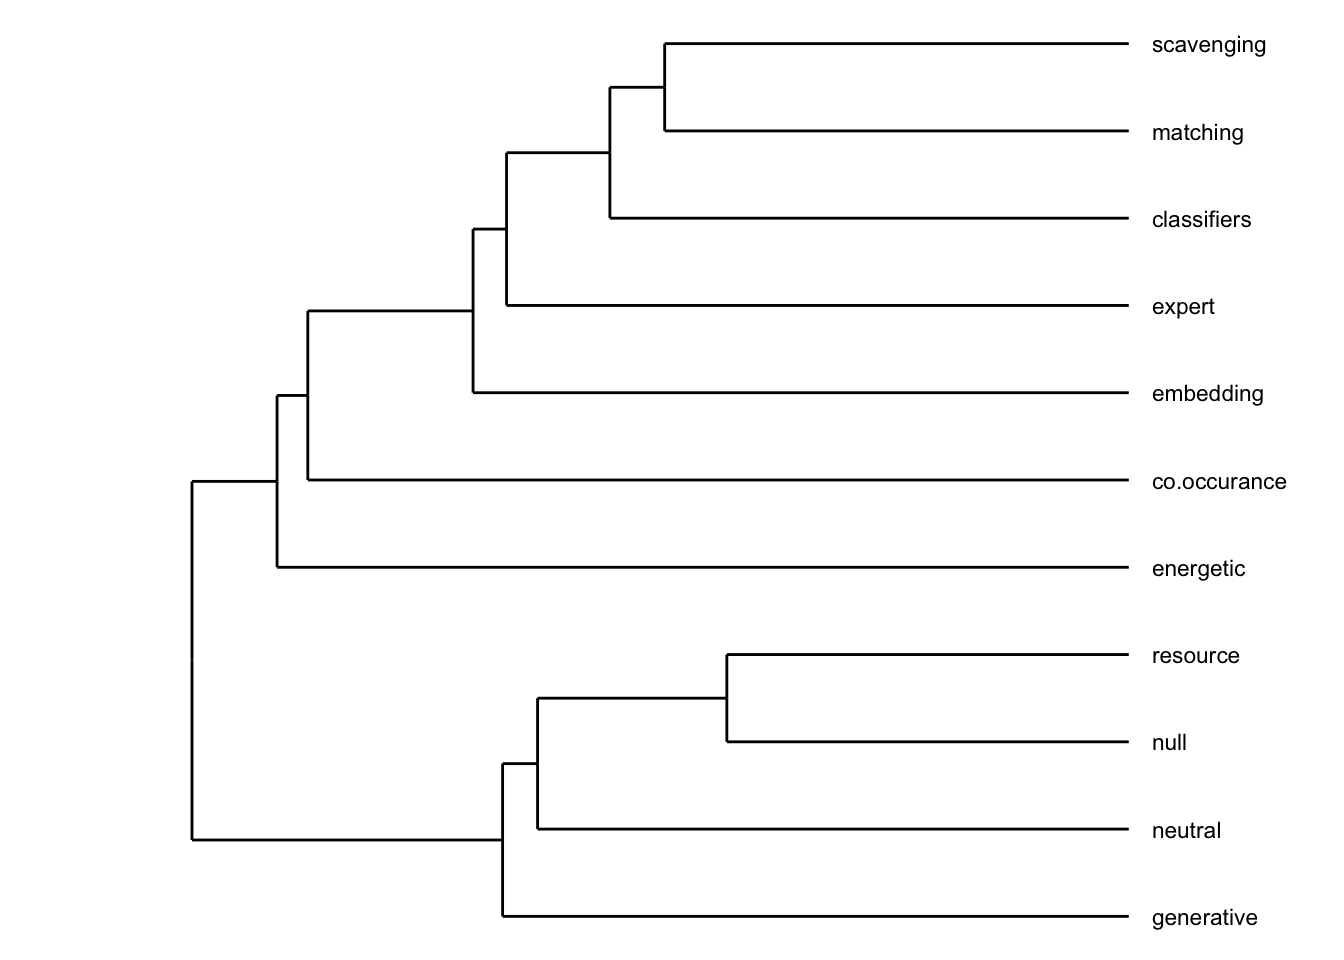
\includegraphics{index_files/figure-latex/notebooks-model_qualitative-fig-dendo-output-1.png}

}

\caption{\label{fig-dendo}Dendrogram of the trait table}

\end{figure}%

\textsubscript{Source:
\href{https://BecksLab.github.io/ms_t_is_for_topology/notebooks/model_qualitative-preview.html\#cell-fig-dendo}{Model
family traits}}

\subsection{Assessing model outputs}\label{assessing-model-outputs}

Although understanding the underlying philosophy of the different model
families is beneficial it is also important to understand in what
situations the different families are likely to preform well or poorly.
When we are assessing the performance of the different model families it
is beneficial to think of benchmarking these assessments based on a
broader basis than just its ability to correctly recover network
structure or pairwise interactions. When thinking about how to benchmark
models it is perhaps beneficial to take a step back and once again
assess what are the needs of the researcher
(Section~\ref{sec-network-why}) and linking this back to what aspects of
the network (Section~\ref{sec-network-anatomy}) are of importance and
assess the performance of a model within those parameters.

Benchmarking how well a model is doing to capture the desired elements
of a network is also a task that required some thought and
contemplation. Even if we think about the predicting the structure of a
network it is possible that two networks may have the same number of
nodes and links but that those links may be distributed in very
different ways. Thus it is important to think critically about the suite
of summary statistics that are used to assess a model, since there is no
one `silver bullet' summary statistic that will be able to assess if a
model is able to fully replicate an empirical network {[}26{]}. One of
the main challenges when assessing the ability to retrieve pairwise
interactions is that food webs are sparse (that means that there are few
links given the number of species) and it is important that we are able
to discern between a model that is able to correctly predict
interactions that do (true positives) and not (true negatives) occur and
one that is simply predicting a lack of interactions {[}29{]}.

\paragraph{Benchmarking for structure}\label{benchmarking-for-structure}

Despite structural models being some of the older model families there
is a distinctive lack of clear guidelines as to how we assess the
ability of these models to replicate the \emph{entire} structure of a
network. In part this may perhaps be driven by the underlying research
agenda and interest in different aspects of capturing the structure of
networks \emph{e.g.,} the obsession with intervality {[}ref{]} or link
distributions {[}ref{]}. However, it is still a good idea to think about
the network in its entirety and to benchmark structural models in a more
holistic manner. Some useful ways to assess how well the model predicts
the shape (\emph{e.g.,} the height (chain length) and\ldots), links
(\emph{e.g.,} connectance), internal structure (\emph{e.g.,} SVD
entropy, {[}30{]}), and meso-level features (\emph{e.g.,} motifs,
{[}31{]}) of a network. This is shown in
Figure~\ref{fig-topology}\ldots{}

\begin{itemize}
\item
  Maybe look at some of the historic papers that compare some of the
  `resource models'
\item
  See also {[}26{]} and the likelihood function that they use for model
  selection
\item
  Look at {[}32{]}
\end{itemize}

\begin{figure}[H]

\centering{

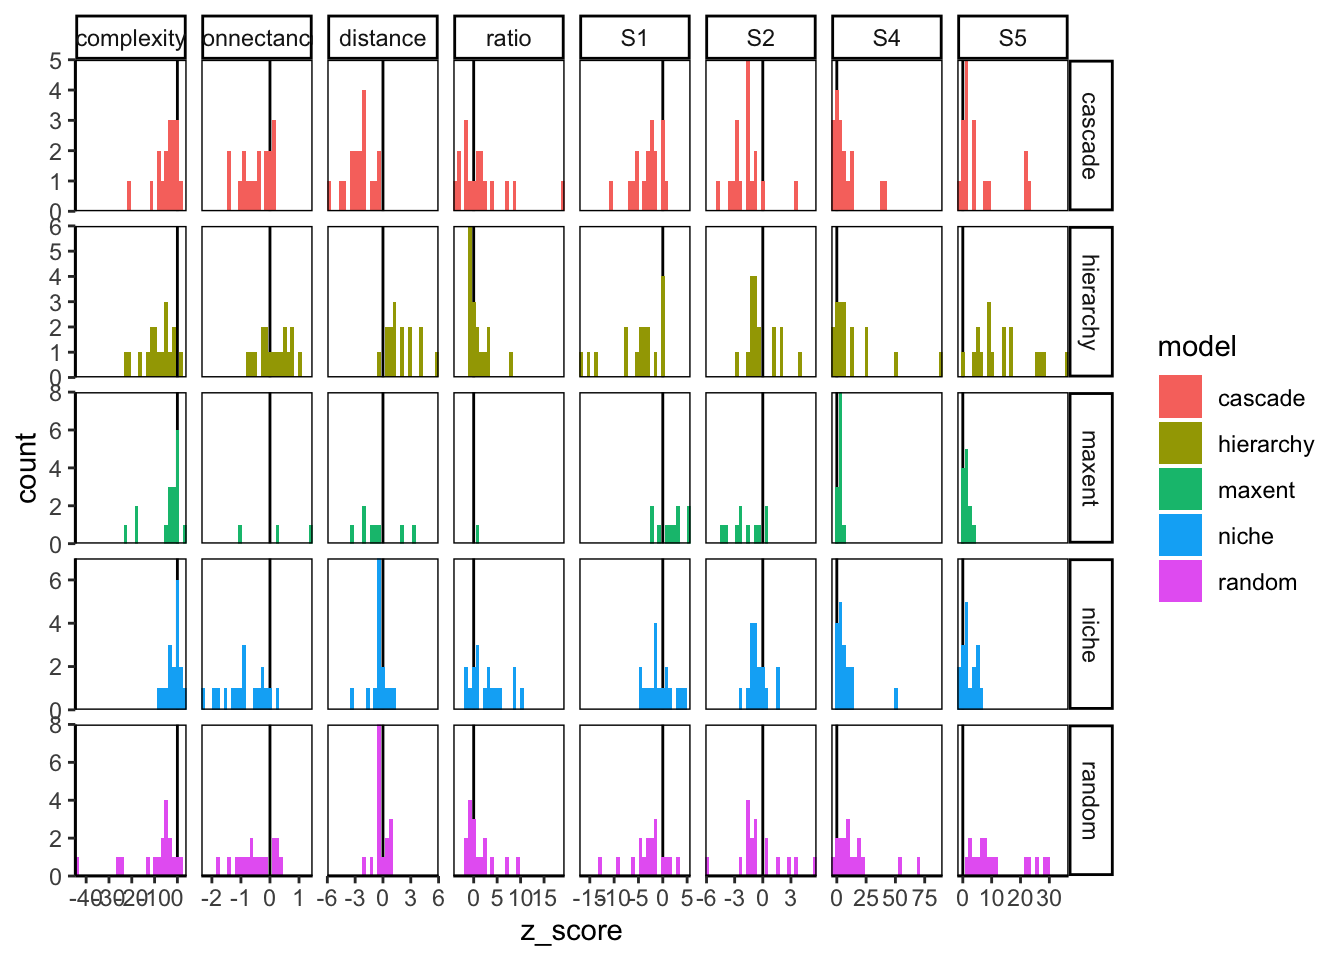
\includegraphics{index_files/figure-latex/notebooks-model_quantitative-fig-topology-output-2.png}

}

\caption{\label{fig-topology}Difference between real and model network
property. S1 - S5 represent the different motif structures identified in
{[}31{]}.}

\end{figure}%

\textsubscript{Source:
\href{https://BecksLab.github.io/ms_t_is_for_topology/notebooks/model_quantitative-preview.html\#cell-fig-topology}{Quantitative
approach to topology generators}}

\paragraph{Benchmarking for
interactions}\label{benchmarking-for-interactions}

Broadly speaking the task of assessing the ability of a model to predict
interactions as being an assessment of the model's classification
ability (does it correctly predict the presence and absence of
interactions?) and so we want to benchmark the model on how well it is
able to correctly predict these presences and absences. This can be done
in a myriad of ways {[}9,29{]} but is always based off of the confusion
matrix. Using the confusion matrix it is then possible to assess the
`quality' of the model predictions such as their accuracy or
informedness. The high class imbalance (inherit sparsity) of networks
means that most interactions are absent and so a model that predicts
interactions as being absent will still predict most interactions
correctly {[}\emph{i.e.,} getting the `right' answers but for the wrong
reasons, 29{]}

\begin{itemize}
\item
  As per {[}29{]} the best ways to assess the classification performance
  of the different models is to use the Precision-Recall (PR-AUC) to
  assess precision {[}ref?{]}, and the Matthews correlation coefficient
  (MCC) to assess accuracy {[}33{]}.
\item
  Caveat regarding the use of real world interaction data both for
  training and validating predictions? \emph{e.g.,} Poisot, Ouellet, et
  al.~et al 2021 and Catchen et al 2023
\item
  ``These results suggest that learning from a dataset with very low
  connectance can be a different task than for more connected networks:
  it becomes increasingly important to capture the mechanisms that make
  an interaction exist, and therefore having a slightly more biased
  training dataset might be beneficial. As connectance increases, the
  need for biased training sets is less prominent, as learning the rules
  for which interactions do not exist starts gaining importance''
\item
  Maybe also looking at how well a model can recover `missing links'
  \emph{i.e.,} introducing false negatives into the training data
  \emph{sensu} what we did in {[}34{]}
\end{itemize}

\begin{figure}

\centering{

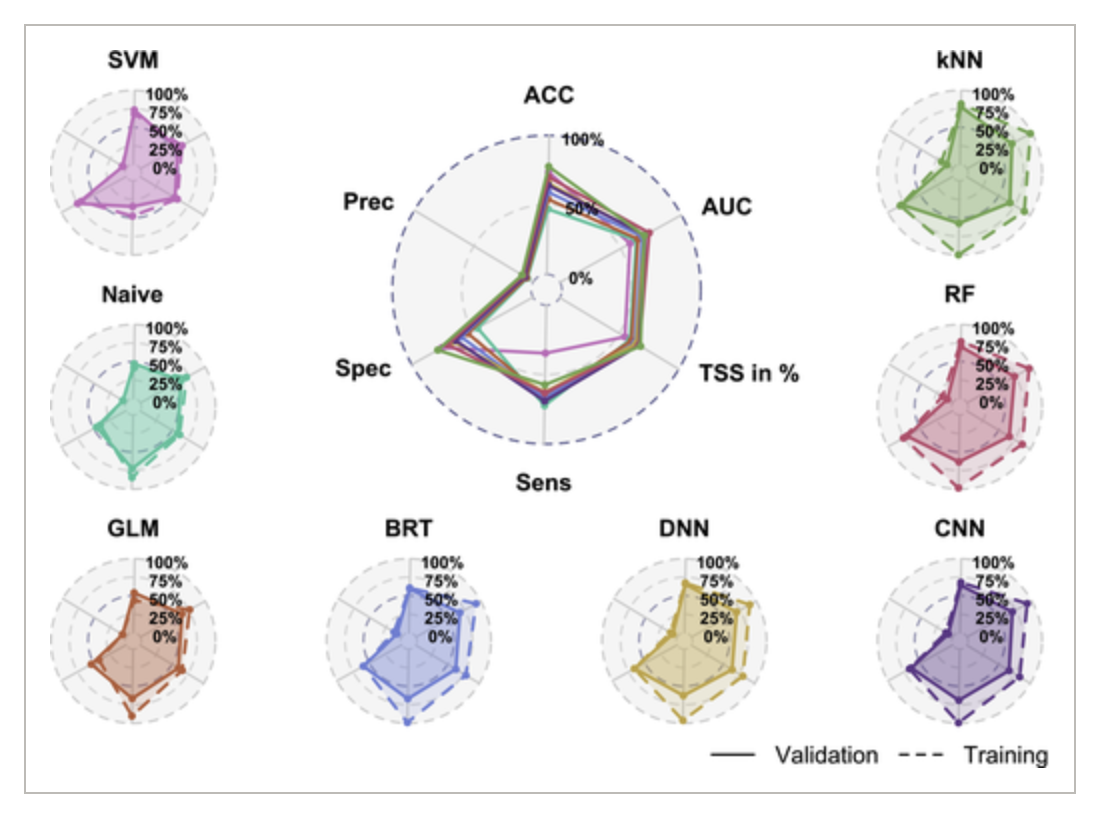
\includegraphics{images/pichler_result.png}

}

\caption{\label{fig-pichler}Moc result from {[}5{]}}

\end{figure}%

\subsection{The bigger picture}\label{the-bigger-picture}

In addition to thinking about the `performance' if a model it is also
important to be aware of the `unseen' costs and limitations of the
different modelling families. What data do I need? Can a make \emph{de
novo} predictions? What are the related `sinks' \emph{e.g.,}
computational or time? What does the network I am constructing actually
represent?

\subsubsection{Data need vs
availability}\label{data-need-vs-availability}

This includes thinking about the need for additional data sources (such
as trait or phylogenetic data), the computational cost, as well as the
time it might take to generate a network, \emph{e.g.,} binary
classifiers require an (often times) extensive list of additional trait
data for the model training process, which limits predictions to
communities for which you do have the relevant auxiliary data available.

\subsubsection{Theory vs `real world'}\label{theory-vs-real-world}

Probably mentioned elsewhere but basically are we constructing networks
because we want to make real-world, case-specific predictions
\emph{e.g.,} for a conservation area or do we want to just have a set of
ecologically plausible networks we can use for theoretical stuffs. Need
to discuss the key differences and implications between predicting a
metaweb (\emph{sensu} {[}20{]}) and a network realisation. (In a way the
idea of predicting a metaweb vs realisation is what makes me hesitant to
use the Mangal networks to test the structural models because do we even
know what the Mangal networks represent and what the structural models
are predicting\ldots) Maybe also {[}35{]} that discuss how the local
factors are going to play a role.

\subsubsection{The target system?}\label{the-target-system}

\subsubsection{Philosophy limits theory}\label{philosophy-limits-theory}

Also need to take into consideration inherent constraints that the model
imposes on itself and how it will affect our ability to test
hypotheses/ask questions using the \emph{e.g.,} from {[}36{]} - models
that are constrained by connectance means that we are unable to explain
connectance itself and you would need a different approach if
understanding connectance is your goal. Another way of phrasing this is
thinking about what is needed (input data/parameters), produced (final
network characteristics), and desired (end-use).

\section{Concluding remarks}\label{concluding-remarks}

\begin{itemize}
\item
  Bring up the fact that delimiting a network is in and of itself fuzzy
  - we tend to think of them in terms of snapshots but in reality the
  final (empirical) network is often the result of aggregation over
  multiple timescales.
\item
  Also the fact that \emph{some} people are concerned about the
  taxonomic resolution and cascading effects those might have on our
  understanding of network structure {[}7,19{]}, we are at risk of
  losing our ability to distinguish the wood from the tree - are we not
  (at least at times) concerned more with understanding ecosystem level
  processes than with needing to understand things \emph{perfectly} at
  the species level.

  \begin{itemize}
  \tightlist
  \item
    I don't think these `rare'/nuanced links (e.g.~carnivorous hippos)
    are going to rock the boat when we think about networks at the
    structural level. To say this in a different way maybe it comes down
    to thinking about the scale of organisation within a network\ldots{}
    The classical levels of organisation within ecology (population,
    community, \ldots) are also relevant when we think about a networks.
  \end{itemize}
\item
  In certain situations structure is `enough' but there may be use cases
  where we are really interested in the node-level interactions
  \emph{i.e.,} species identity is a thing we care about and need to be
  able to retrieve specific interactions at specific nodes correctly.
\item
  What is the purpose of generating a network? Is it an element of a
  bigger question we are asking, \emph{e.g.,} I want to generate a
  series of networks to do some extinction simulations/bioenergetic
  stuff OR are we looking for a `final product' network that is relevant
  to a specific location? (this can still be broad in geographic scope).
\end{itemize}

Interestingly {[}4{]} also explicitly talk about \emph{structural}
food-web models in their introduction\ldots{} so how I see it that means
that there has always been this inherent acknowledgement that models are
functioning at a specific `network level'.

\begin{quote}
``The resolution of food-web data is demonic because it can radically
change network topology and associated biological inferences in ways
that are unknowable in the absence of better data.'' - {[}7{]} The
counter to this is that structural models are often not working at the
species level and thus the structure remains `unchanged' when you
increase the resolution - I don't think that people are that concerned
with the structure of real world networks barring connectance and since
that scales with species richness anyway your final proportion will
probably still remain the same\ldots{}
\end{quote}

\begin{quote}
``It makes no sense to describe the interaction structure of nodes which
in themselves are poorly defined.'' --- Roslin et al.~(2013, p.~2)
\end{quote}

\begin{itemize}
\item
  I think a big take home will (hopefully) be how different approaches
  do better in different situations and so you as an end user need to
  take this into consideration and pick accordingly. I think {[}36{]}
  might have (and share) some thoughts on this (thanks Andrew). I feel
  like I need to look at {[}37{]} but maybe not exactly in this context
  but vaguely adjacent.
\item
  An interesting thing to also think about (and arguably it will be
  addressed based on some of the other thoughts and ideas) is data
  dependant and data independent `parametrisation' of the models\ldots{}
\item
  Why do interaction models do so badly at predicting structure? Nuance
  of metaweb vs realisation but also time? At the core of it interaction
  models are trained on existing interaction data; this is data that are
  most likely closer to a metaweb than a local realisation even if they
  are being inventoried at a small scale.

  \begin{itemize}
  \tightlist
  \item
    I think this is sort of the crux of the argument presented in
    {[}38{]}
  \end{itemize}
\end{itemize}

\begin{quote}
\emph{``we highlight an interesting paradox: the models with the best
performance measures are not necessarily the models with the closest
reconstructed network structure.''} - {[}29{]}
\end{quote}

\begin{itemize}
\item
  \emph{Do we need network models to predict interactions and
  interaction models to predict structure?} (lets not think about that
  too hard or I might just have to sit in silence for a while\ldots)

  \begin{itemize}
  \item
    ``Another argument for the joint prediction of networks and
    interactions is to reduce circularity and biases in the predictions.
    As an example, models like linear filtering generate probabilities
    of non-observed interactions existing, but do so based on measured
    network properties.'' - {[}9{]}
  \item
    Aligning (dove-tailing) with this the idea of ensemble modelling as
    presented by {[}39{]}
  \end{itemize}
\item
  It will be interesting to bring up the idea that if a model is missing
  a specific pairwise link but doing well at the structural level then
  when does it matter?
\item
  Close out with a call to action that we have models that predict
  networks very well and models that predict interactions very well but
  nothing that is doing well at predicting both - this is where we
  should be focusing our attention when it comes to furthering model
  development. (we need models that will fill the space in the top right
  quadrant of panel A in Figure~\ref{fig-concept})
\end{itemize}

\subsection{Downsampling}\label{downsampling}

\begin{itemize}
\item
  {[}40{]}
\item
  ``That being said, there is a compelling argument for the need to
  `combine' these smaller functional units with larger spatial networks
  {[}41{]} and that we should also start thinking about the interplay of
  time and space {[}42{]}. Although deciding exactly what measure might
  actually be driving differences between local networks and the
  regional metaweb might not be that simple {[}43{]}.''
\end{itemize}

\section*{Glossary}\label{glossary}
\addcontentsline{toc}{section}{Glossary}

\begin{longtable}[]{@{}
  >{\raggedright\arraybackslash}p{(\columnwidth - 2\tabcolsep) * \real{0.5000}}
  >{\raggedright\arraybackslash}p{(\columnwidth - 2\tabcolsep) * \real{0.5000}}@{}}
\toprule\noalign{}
\begin{minipage}[b]{\linewidth}\raggedright
Term
\end{minipage} & \begin{minipage}[b]{\linewidth}\raggedright
Definition
\end{minipage} \\
\midrule\noalign{}
\endhead
\bottomrule\noalign{}
\endlastfoot
food web & a representation of feeding links between species \\
network generator & a model that predicts a network based on assumptions
of structure, this network is species agnostic in the sense that it does
not necessarily contain information at the node level \\
interaction predictor & a model that predicts species interactions,
these interactions can be used to construct a network but there are no
\emph{a priori} assumptions as that will constrain the network
structure \\
model & A tool that can be used to construct food webs, where the
resulting network is a representation of a real world network. Models
typically only capture specific elements of real world networks and are
intended to be used in specific settings \\
model family & A family of models that share an underlying philosophy
when it comes to the mapping, pragmatism, and reduction of a network.
Families have the same underlying philosophies and assumptions that
determine the links between nodes as well as how these may be encoded \\
metaweb & A network that represents \emph{all} the potential links
between species. Importantly these links will not necessarily all be
realised in a specific location for a specific time \\
realised network & A network that represents the links between species
that are occurring. These networks represent a very localised
network\ldots{} \\
potential feeding link & links that indicate that an interaction is
ecologically feasible but not realised \emph{per se} (a metaweb would
contain potential feeding links) \\
realised feeding link & links that indicate that the interaction is
realised `in the field'. (a realised network contains realised feeding
links) \\
confusion matrix & captures the number of true positives (interaction
predicted as present when it is present), false negatives (interaction
predicted as absent when it is present), false positives (interaction
predicted as present when it is absent), and true negatives (interaction
predicted as absent when it is absent) \\
\end{longtable}

\section*{Outstanding questions}\label{outstanding-questions}
\addcontentsline{toc}{section}{Outstanding questions}

\begin{itemize}
\tightlist
\item
  non-consumptive effects
\end{itemize}

\section*{References}\label{references}
\addcontentsline{toc}{section}{References}

\phantomsection\label{refs}
\begin{CSLReferences}{0}{0}
\bibitem[\citeproctext]{ref-poisotGlobalKnowledgeGaps2021}
\CSLLeftMargin{1. }%
\CSLRightInline{Poisot, T. \emph{et al.} (2021)
\href{https://doi.org/10.1111/jbi.14127}{Global knowledge gaps in
species interaction networks data}. \emph{Journal of Biogeography} n/a}

\bibitem[\citeproctext]{ref-jordanoChasingEcologicalInteractions2016}
\CSLLeftMargin{2. }%
\CSLRightInline{Jordano, P. (2016)
\href{https://doi.org/10.1371/journal.pbio.1002559}{Chasing {Ecological
Interactions}}. \emph{PLOS Biology} 14, e1002559}

\bibitem[\citeproctext]{ref-jordanoSamplingNetworksEcological2016}
\CSLLeftMargin{3. }%
\CSLRightInline{Jordano, P. (2016) Sampling networks of ecological
interactions. \emph{Functional Ecology} DOI:
\href{https://doi.org/10.1111/1365-2435.12763}{10.1111/1365-2435.12763}}

\bibitem[\citeproctext]{ref-williamsSuccessItsLimits2008}
\CSLLeftMargin{4. }%
\CSLRightInline{Williams, R.J. and Martinez, N.D. (2008)
\href{https://doi.org/10.1111/j.1365-2656.2008.01362.x}{Success and its
limits among structural models of complex food webs}. \emph{Journal of
Animal Ecology} 77, 512--519}

\bibitem[\citeproctext]{ref-pichlerMachineLearningAlgorithms2020}
\CSLLeftMargin{5. }%
\CSLRightInline{Pichler, M. \emph{et al.} (2020)
\href{https://doi.org/10.1111/2041-210X.13329}{Machine learning
algorithms to infer trait-matching and predict species interactions in
ecological networks}. \emph{Methods in Ecology and Evolution} 11,
281--293}

\bibitem[\citeproctext]{ref-darwinOriginSpeciesMeans1859}
\CSLLeftMargin{6. }%
\CSLRightInline{Darwin, C. (1859) \emph{On the {Origin} of {Species} by
{Means} of {Natural Selection}, or the {Preservation} of {Favoured
Races} in the {Struggle} for {Life}}, J. Murray}

\bibitem[\citeproctext]{ref-pringleResolvingFoodWebStructure2020}
\CSLLeftMargin{7. }%
\CSLRightInline{Pringle, R.M. and Hutchinson, M.C. (2020)
\href{https://doi.org/10.1146/annurev-ecolsys-110218-024908}{Resolving
{Food-Web Structure}}. \emph{Annual Review of Ecology, Evolution and
Systematics} 51, 55--80}

\bibitem[\citeproctext]{ref-morales-castillaInferringBioticInteractions2015}
\CSLLeftMargin{8. }%
\CSLRightInline{Morales-Castilla, I. \emph{et al.} (2015)
\href{https://doi.org/10.1016/j.tree.2015.03.014}{Inferring biotic
interactions from proxies}. \emph{Trends in Ecology \& Evolution} 30,
347--356}

\bibitem[\citeproctext]{ref-strydomRoadmapPredictingSpecies2021}
\CSLLeftMargin{9. }%
\CSLRightInline{Strydom, T. \emph{et al.} (2021)
\href{https://doi.org/10.1098/rstb.2021.0063}{A roadmap towards
predicting species interaction networks (across space and time)}.
\emph{Philosophical Transactions of the Royal Society B: Biological
Sciences} 376, 20210063}

\bibitem[\citeproctext]{ref-poisotSyntheticDatasetsCommunity2016}
\CSLLeftMargin{10. }%
\CSLRightInline{Poisot, T. \emph{et al.} (2016)
\href{https://doi.org/10.1111/ecog.01941}{Synthetic datasets and
community tools for the rapid testing of ecological hypotheses}.
\emph{Ecography} 39, 402--408}

\bibitem[\citeproctext]{ref-daleGraphsSpatialGraphs2010}
\CSLLeftMargin{11. }%
\CSLRightInline{Dale, M.R.T. and Fortin, M.-J. (2010)
\href{https://www.jstor.org/stable/27896212}{From {Graphs} to {Spatial
Graphs}}. \emph{Annual Review of Ecology, Evolution, and Systematics}
41, 21--38}

\bibitem[\citeproctext]{ref-fortinSpatialStatisticsSpatial2012}
\CSLLeftMargin{12. }%
\CSLRightInline{Fortin, M.-J. \emph{et al.} (2012)
\href{https://doi.org/10.1016/j.spasta.2012.02.004}{Spatial statistics,
spatial regression, and graph theory in ecology}. \emph{Spatial
Statistics} 1, 100--109}

\bibitem[\citeproctext]{ref-delmasAnalysingEcologicalNetworks2019}
\CSLLeftMargin{13. }%
\CSLRightInline{Delmas, E. \emph{et al.} (2019)
\href{https://doi.org/10.1111/brv.12433}{Analysing ecological networks
of species interactions}. \emph{Biological Reviews} 94, 16--36}

\bibitem[\citeproctext]{ref-thuillerNavigatingIntegrationBiotic2024}
\CSLLeftMargin{14. }%
\CSLRightInline{Thuiller, W. \emph{et al.} (2024)
\href{https://doi.org/10.1111/jbi.14734}{Navigating the integration of
biotic interactions in biogeography}. \emph{Journal of Biogeography} 51,
550--559}

\bibitem[\citeproctext]{ref-bhatiaNetworkbasedRestorationStrategies2023}
\CSLLeftMargin{15. }%
\CSLRightInline{Bhatia, U. \emph{et al.} (2023)
\href{https://doi.org/10.1038/s42003-023-05622-3}{Network-based
restoration strategies maximize ecosystem recovery}.
\emph{Communications Biology} 6, 1--10}

\bibitem[\citeproctext]{ref-poisotDescribeUnderstandPredict2016}
\CSLLeftMargin{16. }%
\CSLRightInline{Poisot, T. \emph{et al.} (2016)
\href{https://www.jstor.org/stable/48582345}{Describe, understand and
predict: Why do we need networks in ecology?} \emph{Functional Ecology}
30, 1878--1882}

\bibitem[\citeproctext]{ref-proulxNetworkThinkingEcology2005}
\CSLLeftMargin{17. }%
\CSLRightInline{Proulx, S.R. \emph{et al.} (2005)
\href{https://doi.org/10.1016/j.tree.2005.04.004}{Network thinking in
ecology and evolution}. \emph{Trends in Ecology \& Evolution} 20,
345--353}

\bibitem[\citeproctext]{ref-brimacombeShortcomingsReusingSpecies2023}
\CSLLeftMargin{18. }%
\CSLRightInline{Brimacombe, C. \emph{et al.} (2023)
\href{https://doi.org/10.1371/journal.pbio.3002068}{Shortcomings of
reusing species interaction networks created by different sets of
researchers}. \emph{PLOS Biology} 21, e3002068}

\bibitem[\citeproctext]{ref-pringleUntanglingFoodWebs2020}
\CSLLeftMargin{19. }%
\CSLRightInline{Pringle, R.M. (2020)
\href{https://doi.org/10.1515/9780691195322-020}{Untangling {Food
Webs}}. In \emph{Untangling {Food Webs}}, pp. 225--238, Princeton
University Press}

\bibitem[\citeproctext]{ref-dunneNetworkStructureFood2006}
\CSLLeftMargin{20. }%
\CSLRightInline{Dunne, J.A. (2006) The {Network Structure} of {Food
Webs}. In \emph{Ecological networks: {Linking} structure and dynamics}
(Dunne, J. A. and Pascual, M., eds), pp. 27--86, Oxford University
Press}

\bibitem[\citeproctext]{ref-lindemanTrophicDynamicAspectEcology1942}
\CSLLeftMargin{21. }%
\CSLRightInline{Lindeman, R.L. (1942)
\href{https://doi.org/10.2307/1930126}{The {Trophic-Dynamic Aspect} of
{Ecology}}. \emph{Ecology} 23, 399--417}

\bibitem[\citeproctext]{ref-poisotStructureProbabilisticNetworks2016}
\CSLLeftMargin{22. }%
\CSLRightInline{Poisot, T. \emph{et al.} (2016)
\href{https://doi.org/10}{The structure of probabilistic networks}.
\emph{Methods in Ecology and Evolution} 7, 303--312}

\bibitem[\citeproctext]{ref-berlowInteractionStrengthsFood2004}
\CSLLeftMargin{23. }%
\CSLRightInline{Berlow, E.L. \emph{et al.} (2004)
\href{https://doi.org/10.1111/j.0021-8790.2004.00833.x}{Interaction
strengths in food webs: Issues and opportunities}. \emph{Journal of
Animal Ecology} 73, 585--598}

\bibitem[\citeproctext]{ref-cohenStochasticTheoryCommunity1985}
\CSLLeftMargin{24. }%
\CSLRightInline{Cohen, J.E. \emph{et al.} (1985)
\href{https://doi.org/10.1098/rspb.1985.0042}{A stochastic theory of
community food webs {I}. {Models} and aggregated data}.
\emph{Proceedings of the Royal Society of London. Series B. Biological
Sciences} 224, 421--448}

\bibitem[\citeproctext]{ref-cohenFoodWebsDimensionality1977}
\CSLLeftMargin{25. }%
\CSLRightInline{Cohen, J.E. (1977)
\href{https://doi.org/10.1073/pnas.74.10.4533}{Food webs and the
dimensionality of trophic niche space}. \emph{Proceedings of the
National Academy of Sciences} 74, 4533--4536}

\bibitem[\citeproctext]{ref-allesinaGeneralModelFood2008}
\CSLLeftMargin{26. }%
\CSLRightInline{Allesina, S. \emph{et al.} (2008)
\href{https://doi.org/10.1126/science.1156269}{A {General Model} for
{Food Web Structure}}. \emph{Science} 320, 658--661}

\bibitem[\citeproctext]{ref-petcheySizeForagingFood2008}
\CSLLeftMargin{27. }%
\CSLRightInline{Petchey, O.L. \emph{et al.} (2008)
\href{https://doi.org/10.1073/pnas.0710672105}{Size, foraging, and food
web structure}. \emph{Proceedings of the National Academy of Sciences}
105, 4191--4196}

\bibitem[\citeproctext]{ref-strydomGraphEmbeddingTransfer2023}
\CSLLeftMargin{28. }%
\CSLRightInline{Strydom, T. \emph{et al.} (2023)
\href{https://doi.org/10.1111/2041-210X.14228}{Graph embedding and
transfer learning can help predict potential species interaction
networks despite data limitations}. \emph{Methods in Ecology and
Evolution} 14, 2917--2930}

\bibitem[\citeproctext]{ref-poisotGuidelinesPredictionSpecies2023}
\CSLLeftMargin{29. }%
\CSLRightInline{Poisot, T. (2023)
\href{https://doi.org/10.1111/2041-210X.14071}{Guidelines for the
prediction of species interactions through binary classification}.
\emph{Methods in Ecology and Evolution} 14, 1333--1345}

\bibitem[\citeproctext]{ref-strydomSVDEntropyReveals2021}
\CSLLeftMargin{30. }%
\CSLRightInline{Strydom, T. \emph{et al.} (2021)
\href{https://doi.org/10.3389/fevo.2021.623141}{{SVD Entropy Reveals}
the {High Complexity} of {Ecological Networks}}. \emph{Frontiers in
Ecology and Evolution} 9}

\bibitem[\citeproctext]{ref-stoufferEvidenceExistenceRobust2007}
\CSLLeftMargin{31. }%
\CSLRightInline{Stouffer, D.B. \emph{et al.} (2007)
\href{https://doi.org/10.1098/rspb.2007.0571}{Evidence for the existence
of a robust pattern of prey selection in food webs}. \emph{Proceedings
of the Royal Society B: Biological Sciences} 274, 1931--1940}

\bibitem[\citeproctext]{ref-vermaatMajorDimensionsFoodweb2009}
\CSLLeftMargin{32. }%
\CSLRightInline{Vermaat, J.E. \emph{et al.} (2009)
\href{https://www.ncbi.nlm.nih.gov/pubmed/19294932}{Major dimensions in
food-web structure properties.} \emph{Ecology} 90, 278--282}

\bibitem[\citeproctext]{ref-matthewsComparisonPredictedObserved1975}
\CSLLeftMargin{33. }%
\CSLRightInline{Matthews, B.W. (1975)
\href{https://doi.org/10.1016/0005-2795(75)90109-9}{Comparison of the
predicted and observed secondary structure of {T4} phage lysozyme}.
\emph{Biochimica et Biophysica Acta (BBA) - Protein Structure} 405,
442--451}

\bibitem[\citeproctext]{ref-strydomFoodWebReconstruction2022}
\CSLLeftMargin{34. }%
\CSLRightInline{Strydom, T. \emph{et al.} (2022)
\href{https://doi.org/10.1111/2041-210X.13835}{Food web reconstruction
through phylogenetic transfer of low-rank network representation}.
\emph{Methods in Ecology and Evolution} 13, 2838--2849}

\bibitem[\citeproctext]{ref-poisotSpeciesWhyEcological2015}
\CSLLeftMargin{35. }%
\CSLRightInline{Poisot, T. \emph{et al.} (2015)
\href{https://doi.org/10.1111/oik.01719}{Beyond species: Why ecological
interaction networks vary through space and time}. \emph{Oikos} 124,
243--251}

\bibitem[\citeproctext]{ref-petcheyFitEfficiencyBiology2011}
\CSLLeftMargin{36. }%
\CSLRightInline{Petchey, O.L. \emph{et al.} (2011)
\href{https://doi.org/10.1016/j.jtbi.2011.03.019}{Fit, efficiency, and
biology: {Some} thoughts on judging food web models}. \emph{Journal of
Theoretical Biology} 279, 169--171}

\bibitem[\citeproctext]{ref-berlowGoldilocksFactorFood2008}
\CSLLeftMargin{37. }%
\CSLRightInline{Berlow, E.L. \emph{et al.} (2008)
\href{https://doi.org/10.1073/pnas.0800967105}{The {``{Goldilocks}
factor''} in food webs}. \emph{Proceedings of the National Academy of
Sciences} 105, 4079--4080}

\bibitem[\citeproctext]{ref-brimacombeApplyingMethodIts2024}
\CSLLeftMargin{38. }%
\CSLRightInline{Brimacombe, C. \emph{et al.} (2024)
\href{https://doi.org/10.13140/RG.2.2.22076.65927}{Applying a method
before its proof-of-concept: {A} cautionary tale using inferred food
webs}}

\bibitem[\citeproctext]{ref-beckerOptimisingPredictiveModels2022}
\CSLLeftMargin{39. }%
\CSLRightInline{Becker, D.J. \emph{et al.} (2022)
\href{https://doi.org/10.1016/S2666-5247(21)00245-7}{Optimising
predictive models to prioritise viral discovery in zoonotic reservoirs}.
\emph{The Lancet Microbe} 3, e625--e637}

\bibitem[\citeproctext]{ref-dansereauSpatiallyExplicitPredictions2023}
\CSLLeftMargin{40. }%
\CSLRightInline{Dansereau, G. \emph{et al.} (2023) Spatially explicit
predictions of food web structure from regional level data}

\bibitem[\citeproctext]{ref-fortinNetworkEcologyDynamic2021}
\CSLLeftMargin{41. }%
\CSLRightInline{Fortin, M.-J. \emph{et al.} (2021)
\href{https://doi.org/10.1098/rspb.2020.1889}{Network ecology in dynamic
landscapes}. \emph{Proceedings of the Royal Society B: Biological
Sciences} 288, rspb.2020.1889, 20201889}

\bibitem[\citeproctext]{ref-estayEditorialPatternsProcesses2023}
\CSLLeftMargin{42. }%
\CSLRightInline{Estay, S.A. \emph{et al.} (2023) Editorial: {Patterns}
and processes in ecological networks over space. \emph{Frontiers in
Ecology and Evolution} 11}

\bibitem[\citeproctext]{ref-saraviaEcologicalNetworkAssembly2022}
\CSLLeftMargin{43. }%
\CSLRightInline{Saravia, L.A. \emph{et al.} (2022)
\href{https://doi.org/10.1111/1365-2656.13652}{Ecological network
assembly: {How} the regional metaweb influences local food webs}.
\emph{Journal of Animal Ecology} 91, 630--642}

\end{CSLReferences}




\end{document}
